\documentclass[journal,12pt,onecolumn]{IEEEtran}
\usepackage{cite}
\usepackage{caption}
\usepackage{graphicx}
\usepackage{amsmath,amssymb,amsfonts,amsthm}
\usepackage{algorithmic}
\usepackage{graphicx}
\usepackage{textcomp}
\usepackage{xcolor}
\usepackage{tfrupee}
\usepackage{txfonts}
\usepackage{listings}
\usepackage{enumitem}
\usepackage{mathtools}
\usepackage{gensymb}
\usepackage{comment}
\usepackage[breaklinks=true]{hyperref}
\usepackage{tkz-euclide} 
\usepackage{listings}
\usepackage{gvv}
%\def\inputGnumericTable{}
\usepackage[latin1]{inputenc} 
\usetikzlibrary{arrows.meta, positioning}
\usepackage{xparse}
\usepackage{color}                                            
\usepackage{array}                                            
\usepackage{longtable}                                       
\usepackage{calc}                                             
\usepackage{multirow}
\usepackage{multicol}
\usepackage{hhline}                                           
\usepackage{ifthen}                                           
\usepackage{lscape}
\usepackage{tabularx}
\usepackage{array}
\usepackage{float}
\usepackage{marvosym}
\usepackage{float}
%\newcommand{\define}{\stackrel{\triangle}{=}}
\theoremstyle{remark}
\usepackage{circuitikz}
\captionsetup{justification=centering}
\usepackage{tikz}

\title{Matrices in Geometry 12.259}
\author{EE25BTECH11037 - Divyansh}
\begin{document}
\vspace{3cm}
\maketitle
{\let\newpage\relax\maketitle}
\textbf{Question: }
Consider the system of equations
\begin{align*}
    \myvec{5 & 2 & 1 \\ -2 & 5 & 2 \\ -1 & 2 & 8}\myvec{x_1 \\ x_2\\ x_3}=\myvec{13 \\ -22 \\ 14}
\end{align*}
With an initial guess of the solution $\myvec{x_1 & x_2& x_3}^{\top} = \myvec{1 & 1& 1}^{\top}$ , the approximate value of the solution $\myvec{x_1 & x_2& x_3}^{\top}$ after one iteration of the Gauss-Seidel method is
\begin{enumerate}
    \item $\myvec{2 & -4.4& 1.625}^{\top}$
    \item $\myvec{2 & 4.4& 1.625}^{\top}$
    \item $\myvec{2 & -4& -3}^{\top}$
    \item $\myvec{2 & -4& 3}^{\top}$
\end{enumerate}
    

\vspace{2mm}


\textbf{Solution:}
Let the initial guess of the solution be 
\begin{align}
    \myvec{x_1 \\ x_2\\ x_3}=\myvec{1 \\1 \\1}
\end{align}
Isolating each variable from the given equations 
\begin{align}
    x_1=\dfrac{13-2x_2-x_3}{5} \ , \ 
    x_2=\dfrac{-22+2x_1-2x_3}{5} \ , \ 
    x_3=\dfrac{14+x_1-2x_2}{8}
\end{align}
Substituting $x_2=1, x_3=1$ in the first equation
\begin{align}
    x_1=\dfrac{13-2-1}{5} = \dfrac{10}{5} =2
\end{align}
Substituting $x_1=2 , x_3=1$ in the second equation
\begin{align}
    x_2=\dfrac{-22+4 -2}{5} = \dfrac{-20}{5} =-4
\end{align}
Substituting $x_1=2, x_2 = -4$
\begin{align}
    x_3=\dfrac{14+2+8}{8}=\dfrac{24}{8}=3
\end{align}
After one iteration of the Gauss-Seidel method, we get
\begin{align}
    \myvec{x_1 \\ x_2 \\ x_3 }=\myvec{2 \\ -4 \\ 3}
\end{align}
which is option $4)$\\
Plotting these points in a graph
\begin{figure}
    \centering
    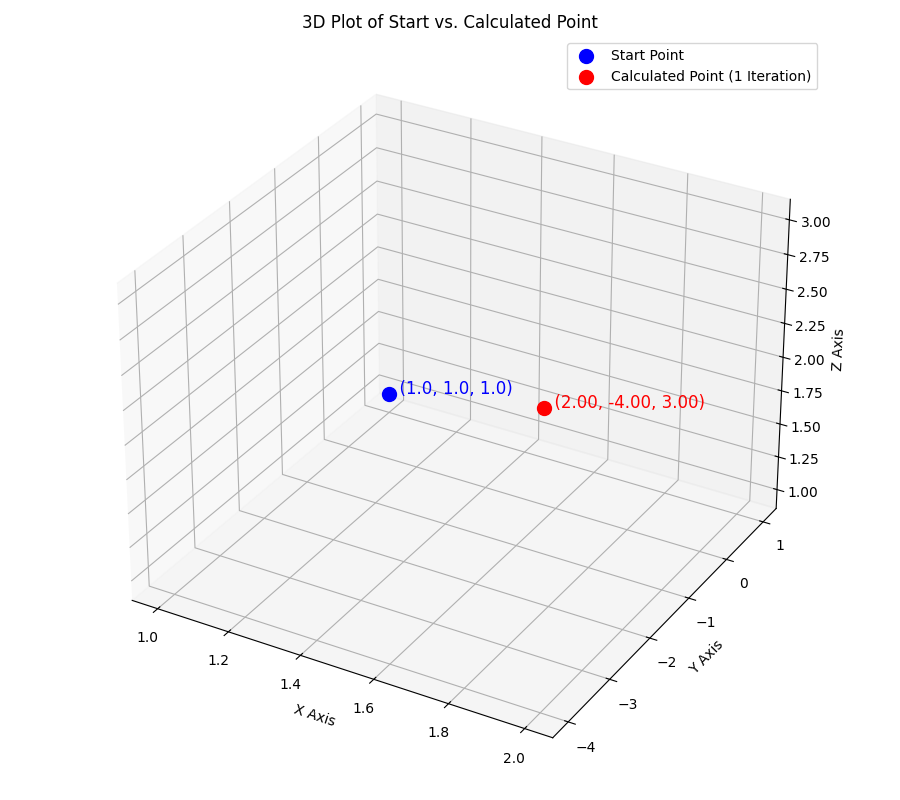
\includegraphics[width=0.5\columnwidth]{figs/1.png}
    \caption{Graph for 12.259}
    \label{fig:placeholder}
\end{figure}
\end{document}
